\documentclass[a4paper,12pt]{article}
%%%%%%%%%%%%%%%%%%%%%%%%%%%%%%%%%%%%%%%%%%%%%%%%%%%%%%%%%%%%%%%%%%%%%%%%%%%%%%%%%%%%%%%%%%%%%%%%%%%%%%%%%%%%%%%%%%%%%%%%%%%%%%%%%%%%%%%%%%%%%%%%%%%%%%%%%%%%%%%%%%%%%%%%%%%%%%%%%%%%%%%%%%%%%%%%%%%%%%%%%%%%%%%%%%%%%%%%%%%%%%%%%%%%%%%%%%%%%%%%%%%%%%%%%%%%
\usepackage{eurosym}
\usepackage{vmargin}
\usepackage{amsmath}
\usepackage{graphics}
\usepackage{epsfig}
\usepackage{enumerate}
\usepackage{multicol}
\usepackage{subfigure}
\usepackage{fancyhdr}
\usepackage{listings}
\usepackage{framed}
\usepackage{graphicx}
\usepackage{amsmath}
\usepackage{chngpage}
%\usepackage{bigints}

\usepackage{vmargin}
% left top textwidth textheight headheight
% headsep footheight footskip
\setmargins{2.0cm}{2.5cm}{16 cm}{22cm}{0.5cm}{0cm}{1cm}{1cm}
\renewcommand{\baselinestretch}{1.3}

\setcounter{MaxMatrixCols}{10}

\begin{document}
\large 
\noindent Actuaries in an insurance company have data which have been collected separately
in two different samples. The actuaries are concerned about the validity of the equal
variance assumption between the two underlying populations when carrying out a
two-sample t-test. The two samples are given below:

\begin{center}
\begin{tabular}{|c|c|}
\hline
 Sample 1:     &  21 22 28 27 20 23 26 32 25 21 30\\ \hline
 Sample 2:    & 19 18 38 33 24 39 22 20 28 26 30 \\
 \hline 
\end{tabular}
\end{center}

\subsection*{Exercise 1}

Enter the data into R.



\begin{framed}\begin{verbatim}
## Data entry

sample1 <- c(21, 22, 28, 27, 20, 23, 26, 32, 25, 21, 30)


# sample2 = c(19, 18, 38, 33, 24, 39, 22, 20, 28, 26, 30)

assign("sample2", c(19, 18, 38, 33, 24, 39, 22,
    20, 28, 26, 30))


\end{verbatim}\end{framed}
\newpage 
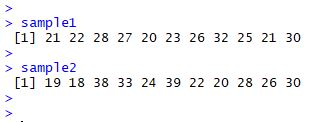
\includegraphics[scale=1.6]{00-A1/images/A1-Q4-Samples.JPG}

\newpage 

\subsection*{Exercise 2}

\noindent Perform an F-test at a 5\% significance level to compare the populationvariances. You should state your conclusion clearly.

$$ H_0 : \sigma^2_{1} = \sigma^2_{2} $$
$$ H_1 : \sigma^2_{1} \neq \sigma^2_{2} $$


\noindent Alternatively, expressed in terms of variance ratios

$$ H_0 : \frac{\sigma^2_{1}}{ \sigma^2_{2} } = 1$$
$$ H_1 : \frac{\sigma^2_{1}}{ \sigma^2_{2} } \neq 1 $$

\newpage 

\begin{framed}\begin{verbatim}
var.test(x = sample1, y = sample2, conf.level = 0.95)

\end{verbatim}\end{framed}


\begin{verbatim}
  
    	F test to compare two variances
    
    data:  sample1 and sample2
    F = 0.29259, num df = 10, denom df = 10, p-value = 0.06553
    alternative hypothesis: true ratio of variances is not equal to 1
    95 percent confidence interval:
     0.07872181 1.08750577
    sample estimates:
    ratio of variances 
             0.2925926 
    
\end{verbatim} 


\newpage 
\begin{framed}\begin{verbatim}
library(broom)
library(magrittr)

var.test(x = sample1, y = sample2, 
    conf.level = 0.95) %>% tidy() 
\end{verbatim}\end{framed}

    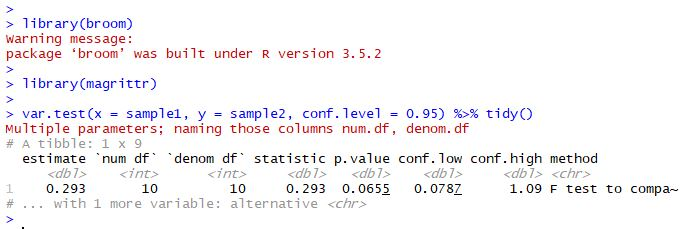
\includegraphics[scale=1.15]{00-A1/images/A1-Q4-Broom.JPG}

\medskip
\noindent The p-value is $0.06553 \geq 0.05$, so we have insufficient evidence to reject the assumption of
equal variance.


\newpage 

\subsection*{Exercise 3}

\noindent Perform a suitable t-test for the null hypothesis that the two population
means are equal at a 5\% significance level.



\begin{framed}\begin{verbatim}
t.test(x = sample1, 
       y = sample2, 
       var.equal = TRUE, 
       conf.level = 0.95)
\end{verbatim}\end{framed}


\begin{verbatim}
    	Two Sample t-test
    
    data:  sample1 and sample2
    t = -0.79396, df = 20, p-value = 0.4365
    alternative hypothesis: true difference in means is not equal to 0
    95 percent confidence interval:
     -7.254581  3.254581
    sample estimates:
    mean of x mean of y 
           25        27  
\end{verbatim}   

\newpage 



\begin{framed}\begin{verbatim}
t.test(x = sample1, 
       y = sample2, 
       var.equal = TRUE, 
       conf.level = 0.95) %>% tidy()


\end{verbatim}\end{framed}


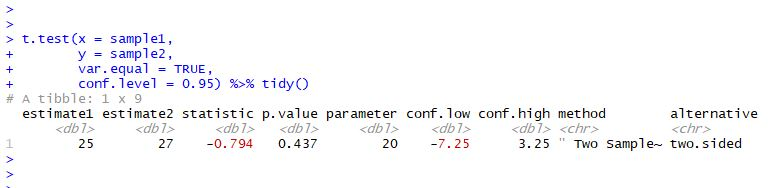
\includegraphics[]{00-A1/images/A1-Q4-Broom2.JPG}


\newpage 
\noindent Calculate a two-sided 95\% confidence interval for the difference in the
population means.



\begin{itemize}
    \item The confidence interval can be read from the previous results or extracted using
\end{itemize}


\begin{framed}\begin{verbatim}

thisTest <- t.test(x = sample1, 
       y = sample2, 
       var.equal = TRUE, 
       conf.level= 0.95)

thisTest$conf.int
\end{verbatim}\end{framed}

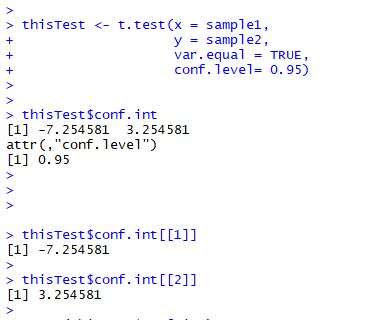
\includegraphics[scale=1.4]{00-A1/images/A1-Q4-ConfInts.JPG}
\begin{itemize}
    \item The 95\% Confidence Interval is (-7.25, 3.25).

\item The p-value of 0.4365 is much larger than the 5\% significance level, therefore we
have no evidence to suggest that the means are different between the two samples.
 
\item It is clear that the confidence interval (-7.25, 3.25) contains 0, therefore 
the assumption of equal means holds.
\end{itemize}




\newpage 

\subsection*{Exercise 4}

\noindent Calculate the two sets of absolute deviations.\\

\noindent [Hint: \texttt{abs(x)} gives the absolute value of x.]
		




\begin{framed}\begin{verbatim}

s1 = abs(sample1 - mean(sample1))

s2 = abs(sample2 - mean(sample2))

\end{verbatim}\end{framed}

\noindent Perform a two-sample t-test on the two sets of absolute deviations at a
5\% level, stating your conclusion.
\newpage 
\begin{framed}\begin{verbatim}

t.test(x = s1, y = s2, 
    var.equal = TRUE, 
    conf.level = 0.95)

\end{verbatim}\end{framed}


\begin{verbatim}
    	Two Sample t-test
    
    data:  s1 and s2
    t = -2.1077, df = 20, p-value = 0.04788
    alternative hypothesis: true difference in means is not equal to 0
    95 percent confidence interval:
     -5.42646442 -0.02808103
    sample estimates:
    mean of x mean of y 
     3.272727  6.000000 

\end{verbatim}    


\newpage 



%%%%%%%%%%%%%%%%%%%%%%%%%%%%%%%%%%%%
\large 

\subsection*{Exercise 5}
\noindent Comment on your conclusions in Exercise 2 and Exercise 4.

\begin{itemize}
    \item A different approach for checking the equal variance assumption between the two
underlying populations is suggested. 

    \item It involves a two-sample t-test: for each sample, calculate the absolute deviations defined as the absolute value of the difference between each observed value and the mean of the sample. 

    \item  Apply a two-sample t-test to the two sets of absolute deviations. 

    \item  The idea is that if the samples have equal variances, then the absolute deviations will have the same mean for both samples.
\end{itemiz e}


%%%%%%%%%%%%%%%%%%%%%%%%%%%%%%%%%%%%
\large 

\subsection*{Exercise 6}

\noindent Comment on whether or not the equality of the population means can still be tested.

\begin{itemize}
    \item The p-value 0.04788 is slightly less than 5\%, so we reject the hypothesis of equal mean of the absolute deviations and therefore the equal variance assumption in the original data.

    \item The tests in Exercise 2 and Exercise 4 give different results but the p-values are quite similar.

    \item We would need to find an appropriate test that allows for the variances to be different
and compare with the tests carried in Exercise 3.
\end{itemize}

\newpage
BLANK

\end{document}
